\section*{Radiation Balance Between Parallel Plates}
Assignment is completed by Mikkel Jaedicke (mijae12) \& Anders Bæk (anbae12)


\begin{equation}
\begin{align*}
m_{ 1 }\frac { { d }^{ 2 } }{ { dt }^{ 2 } } \left[ \begin{matrix} x_{ 1 } \\ y_{ 1 } \end{matrix} \right] &=-\frac { m_{ 1 }\cdot M\cdot g }{ { r }^{ 3 }_{ 1 } } \left[ \begin{matrix} x_{ 1 } \\ y_{ 1 } \end{matrix} \right] +\frac { m_{ 1 }\cdot m_2\cdot g }{ { r }^{ 3 }_{ 12 } } \left[ \begin{matrix} x_{ 2 }-x_{ 1 } \\ y_{ 2 }-y_{ 1 } \end{matrix} \right] \\
m_{ 2 }\frac { { d }^{ 2 } }{ { dt }^{ 2 } } \left[ \begin{matrix} x_{ 1 } \\ y_{ 1 } \end{matrix} \right] &=-\frac { m_{ 2 }\cdot M\cdot g }{ { r }^{ 3 }_{ 2 } } \left[ \begin{matrix} x_{ 1 } \\ y_{ 1 } \end{matrix} \right] -\frac { m_{ 1 }\cdot m_{ 2 }\cdot g }{ { r }^{ 3 }_{ 12 } } \left[ \begin{matrix} x_{ 2 }-x_{ 1 } \\ y_{ 2 }-y_{ 1 } \end{matrix} \right] 
\end{align*}
\label{eq:1}
\end{equation}
where: \( m_1 = m_2 =9.20 \cdot 10^{18} \) [kg], \( M = 5.68  \cdot 10^{26} \) [kg], \( g = 4.98 \cdot 10^{-10} \left[ \frac { \text{km}^3 }{ \text{kg} \cdot \text{døgn} }  \right] \).

\begin{equation}
\begin{align*}
\left[ \begin{matrix} x_{ 1 } \\ y_{ 1 } \end{matrix} \right] &=\left[ \begin{matrix} 0 \\ 152870 \end{matrix} \right] ,\;\;\; 
\frac { d }{ dt } \left[ \begin{matrix} x_{ 1 } \\ y_{ 1 } \end{matrix} \right] =\left[ \begin{matrix} -1360278.1 \\ 0 \end{matrix} \right]  \\
\left[ \begin{matrix} x_{ 2 } \\ y_{ 2 } \end{matrix} \right] &=\left[ \begin{matrix} 0 \\ -153130 \end{matrix} \right] ,\; \;\;
\frac { d }{ dt } \left[ \begin{matrix} x_{ 2 } \\ y_{ 2 } \end{matrix} \right] =\left[ \begin{matrix} 1359122.8 \\ 0 \end{matrix} \right] 
\end{align*}
\label{eq:2}
\end{equation}

\noindent\makebox[\linewidth]{\rule{\textwidth}{0.4pt}}

\section{Pre Calculations}
\todo[inline]{divider med mi fra ligning 1}
\begin{equation}
\begin{align*}
\frac { { d }^{ 2 } }{ { dt }^{ 2 } } \left[ \begin{matrix} x_{ 1 } \\ y_{ 1 } \end{matrix} \right] =-\frac { M\cdot g }{ { r }^{ 3 }_{ 1 } } \left[ \begin{matrix} x_{ 1 } \\ y_{ 1 } \end{matrix} \right] +\frac { m_{ 2 }\cdot g }{ { r }^{ 3 }_{ 12 } } \left[ \begin{matrix} x_{ 2 }-x_{ 1 } \\ y_{ 2 }-y_{ 1 } \end{matrix} \right] \\ 
\frac { { d }^{ 2 } }{ { dt }^{ 2 } } \left[ \begin{matrix} x_{ 1 } \\ y_{ 1 } \end{matrix} \right] =-\frac { M\cdot g }{ { r }^{ 3 }_{ 2 } } \left[ \begin{matrix} x_{ 1 } \\ y_{ 1 } \end{matrix} \right] -\frac { m_{ 1 }\cdot g }{ { r }^{ 3 }_{ 12 } } \left[ \begin{matrix} x_{ 2 }-x_{ 1 } \\ y_{ 2 }-y_{ 1 } \end{matrix} \right] 
\end{align*}
\label{eq:3}
\end{equation}



\begin{equation}
y=\left[ \begin{matrix} x_1\\ y_1\\ x_2\\ y_2\\ \frac { dx_1 }{ dt } \\ \frac { dy_1}{ dt } \\ \frac { dx_2}{ dt } \\ \frac { dy_2 }{ dt } \end{matrix}  \right]
\label{eq:5}
\end{equation}


\begin{equation}
dydx=\left[ \begin{matrix} \frac { -M\cdot g }{ \left( \left( x_{ 1 }^{ 2 }+y_{ 1 }^{ 2 } \right) ^{ 0.5 } \right) ^{ 3 } } \cdot y\left[ 0 \right] +\frac { m_{ 2 }\cdot g }{ \left( \left( \left( x_{ 1 }-x_{ 2 } \right) ^{ 2 }+\left( y_{ 1 }-y_{ 2 } \right) ^{ 2 } \right) ^{ 0.5 } \right)^{ 3 }  } \cdot\left( y\left[ 2 \right] -y\left[ 0 \right]  \right)  \\ \frac { -M\cdot g }{ \left( \left( x_{ 1 }^{ 2 }+y_{ 1 }^{ 2 } \right) ^{ 0.5 } \right) ^{ 3 } } \cdot y\left[ 1 \right] +\frac { m_{ 2 }\cdot g }{ \left( \left( \left( x_{ 1 }-x_{ 2 } \right) ^{ 2 }+\left( y_{ 1 }-y_{ 2 } \right) ^{ 2 } \right) ^{ 0.5 } \right) ^{ 3 } } \cdot \left( y\left[ 3 \right] -y\left[ 1 \right]  \right)  \\ \frac { -M\cdot g }{ \left( \left( x_{ 2 }^{ 2 }+y_{ 2 }^{ 2 } \right) ^{ 0.5 } \right) ^{ 3 } } \cdot y\left[ 2 \right] +\frac { m_{ 1 }\cdot g }{ \left( \left( \left( x_{ 1 }-x_{ 2 } \right) ^{ 2 }+\left( y_{ 1 }-y_{ 2 } \right) ^{ 2 } \right) ^{ 0.5 } \right) ^{ 3 } } \cdot \left( y\left[ 2 \right] -y\left[ 0 \right]  \right)  \\ \frac { -M\cdot g }{ \left( \left( x_{ 2 }^{ 2 }+y_{ 2 }^{ 2 } \right) ^{ 0.5 } \right) ^{ 3 } } \cdot y\left[ 3 \right] +\frac { m_{ 1 }\cdot g }{ \left( \left( \left( x_{ 1 }-x_{ 2 } \right) ^{ 2 }+\left( y_{ 1 }-y_{ 2 } \right) ^{ 2 } \right) ^{ 0.5 } \right) ^{ 3 } } \cdot \left( y\left[ 3 \right] -y\left[ 1 \right]  \right)  \\ 0 \\ 0 \\ 0 \\ 0 \end{matrix} \right] 
\label{eq:6}
\end{equation}




\section{Results of Calculations}

\todo[inline]{omkringskrivning af resultater...}

\begin{equation}
\begin{align*}
r_{ 1 }&=\sqrt { x_{ 1 }^{ 2 }+y_{ 1 }^{ 2 } } \; \text{[km]} \\ 
\theta _{ 1 }&=\arctan { \left( \frac { y_1 }{ x_1 }  \right)  } \; \text{[rad]} \\ 
r_{ 2 }&=\sqrt { x_{ 2 }^{ 2 }+y_{ 2 }^{ 2 } } \; \text{[km]} \\ 
\theta _{ 2 }&=\arctan { \left( \frac { y_2 }{ x_2 }  \right)  } \; \text{[rad]} 
\end{align*}
\label{eq:4}
\end{equation}


\begin{figure}[th!]
\centering
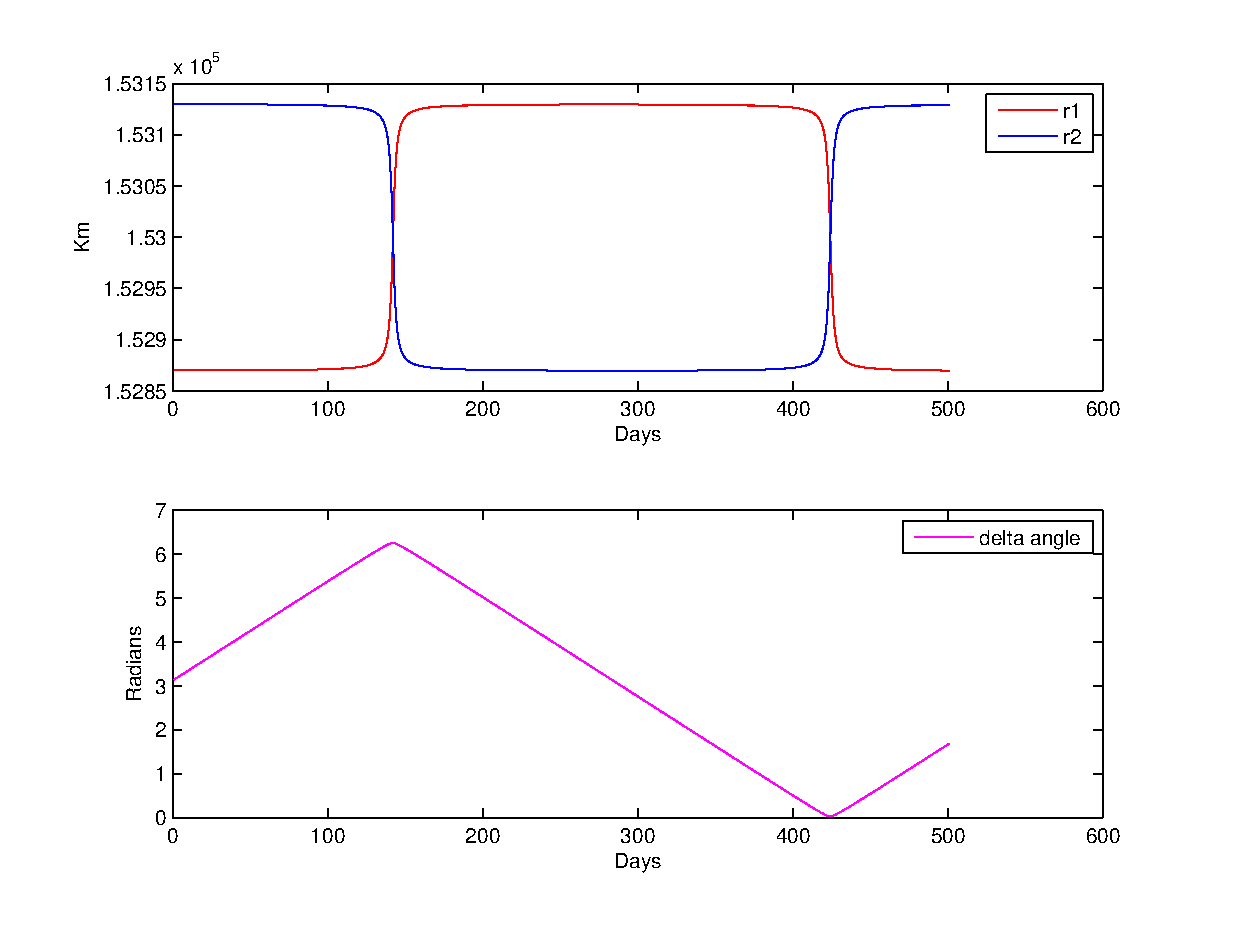
\includegraphics[width=1\textwidth]{./graphics/subplot.eps}
\caption[tekst i indholdsfortegnelsen]{MISSING}
\label{fig:}
\end{figure}

\todo[inline]{kommentar til figuren}
\todo[inline]{nøjagtighed}

